\documentclass[a4paper, 11pt]{article}
\usepackage[AutoFakeBold=true, AutoFakeSlant=true, CJKchecksingle]{xeCJK} 
\usepackage[a4paper]{geometry}
\usepackage{fontspec}
\usepackage{hyperref}
\usepackage{tikz}
\usetikzlibrary{positioning}
\usepackage{subcaption}
\setmainfont{DejaVu Serif}
\setCJKmainfont{Noto Serif CJK TC}
%\XeTeXlinebreaklocale "zh"
% \XeTeXlinebreakskip = 0pt plus 1pt
\begin{document}

\title{红黑树的插入、删除操作之为什么}
\author{tseesing}
\maketitle
红黑树是一种近似平衡的二叉搜索树\footnote{见算法导论第13章},
因其``平衡''(尽管是近似的),其搜索效率比普通二叉搜索树高。既然是``平衡''的,插入、删除
节点时,不可像普通搜索二叉树一般,插入或删除后就撒手不管,红黑树要多做一些工作,以维
持``平衡''。\par 
这个数据结构学习得太痛苦,得作下笔记。难点就在核心的插入、删除节点后为恢复红黑树性质而
作的调整。

红黑树性质\cite{algorithm:intro}(红黑树操作起来复杂,全是为了让整棵树维持着以下这些
性质):\label{properties}
\begin{quote}
\begin{enumerate}
\item 每个节点要么是红色,要么是黑色\label{prop:one}
\item 根节点是黑色\label{prop:two}
\item 每个叶节点(NIL)是黑色\label{prop:three}
\item 如果一个节点是红色的,它的两个孩子必须是黑色\label{prop:four} \footnote{自注:窃以为可理解为父子不
能同红}
\item 任意一个节点,从该节点到其所有后代节点的各个简单路径(simple path),黑色节点的
数目相同(即黑高相同)。\label{prop:five}

\end{enumerate}
\end{quote}

\section{节点变化时为什么要调整?}
为了平衡! 做法就是:将有变化的子树通过旋转、变色操作,使其重新符
合红黑树的5个性质\ref{properties}。

\section{说的``平衡''是什么?}
红黑树性质\ref{prop:five},黑色节点(黑高)相同。每一个节点为根的子树,其左右子树黑高相同:
是为``平衡''。

\section{插入操作相关的为什么}

以下是书本\cite{algorithm:intro}抄出的伪代码(第9行else if 我擅自分成了两行, 方便理解。
另外要吐槽下中译版\cite{algorithm:intro},将伪代码从11行开始分割印到两页上,读者要拿尺
出来量缩进才知道下一页开始时的代码属于哪个block!)

\begin{figure}[h]

\begin{verbatim}
RB-INSERT-FIXUP(T, z)

  1 while z.p.color == RED
  2     if z.p == z.p.p.left
  3         y = z.p.p.right
  4         if y.color == RED
  5             z.p.color = BLACK       // case 1
  6             y.color = BLACK         // case 1
  7             z.p.p.color = RED       // case 1
  8             z = z.p.p               // case 1
  9         else
                if z == z.p.right
 10                 z = z.p             // case 2            
 11                 LEFT-ROTATE(T, z)   // case 2
 12             z.p.color = BLACK       // case 3
 13             z.p.p.color = RED       // case 3
 14             RIGHT-ROTATE(T, z.p.p)  // case 3

 15     else  
            (与 z.p 为 z.p.p 的左孩子的情况对称)

 16 T.root.color = BLACK

\end{verbatim}

\caption{插入节点后恢复红黑树性质的伪代码}
\end{figure}

\begin{figure}[h]
	\centering
	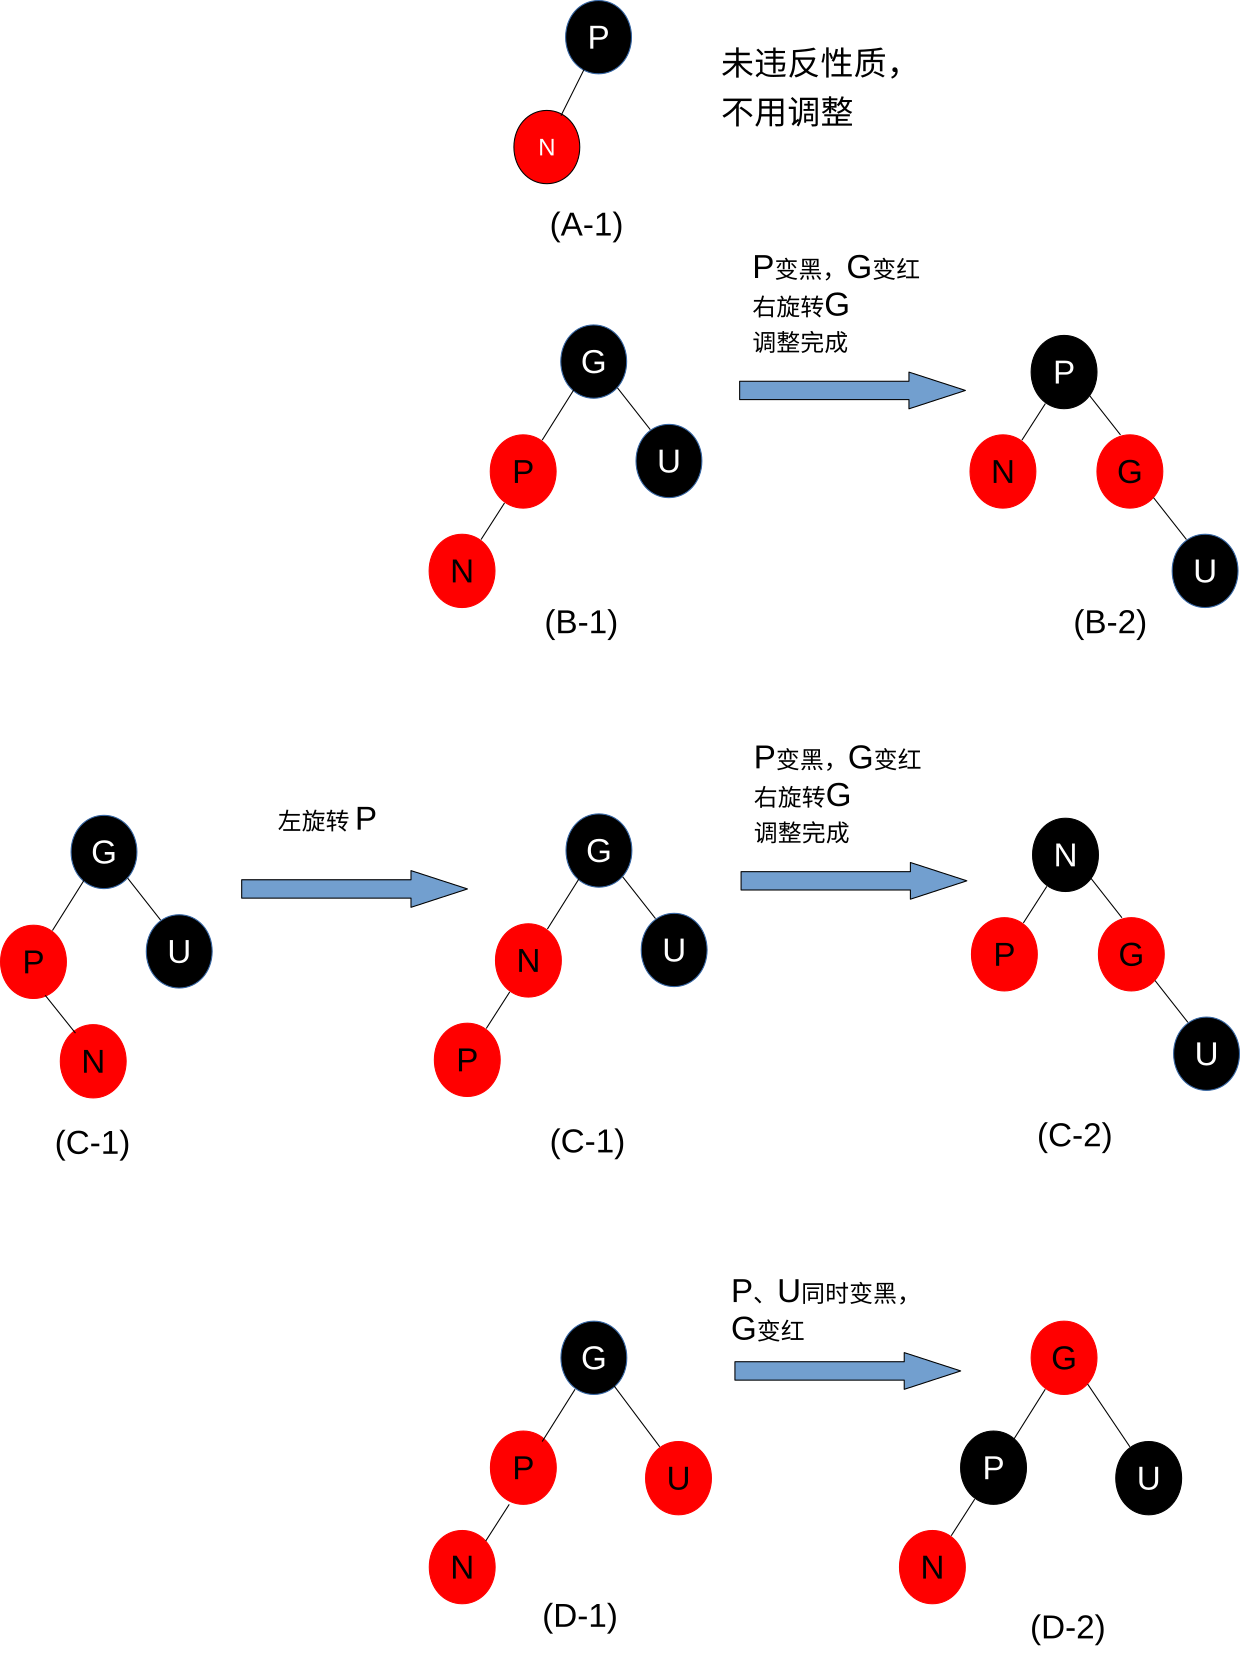
\includegraphics[width=11cm, height=8cm]{images/insert_fixup.png}
	\caption{插入修正过程(N节点为新插入的节点)}
	\label{fig:insert:fixup}
\end{figure}

\subsection{为什么新插入的节点设置成红色?}
《算法导论(第3版)》\cite{algorithm:intro}也问这个问题,我懒,当然不确定自己的想法
是否正确,为了不误导人,直接查到了书中\emph{练习题13.3-1}的答案\cite{book:solution}.
原因就是为了\begin{quote}保持红黑树的性质\ref{prop:five} --- 黑高数目不变!\end{quote}
如果加入的是黑色节点,性质\ref{prop:four}确实不违反;但明显性质会\ref{prop:five}违反。直接不平衡!
如果加入的是红色节点,性质\ref{prop:four}可能违反,但性质\ref{prop:five}却明显不违反!
------ 一个是有可能违反,一个明显违反!

\subsection{插入调整的伪代码是怎么完成调整的?}
新插入的节点Z与父节点P是否同为红色?同就要调整,使其符合性质\ref{prop:four}。
(对照``插入修正过程\ref{fig:insert:fixup}''时,请将图中的N看作Z)。\newline
否则,看叔节点的颜色了,
\begin{itemize}
	
\item 如果叔节点也是红的,就将叔变黑,父 z.p 也变黑,但z.p.p 要变红(相当于z.p.p这个黑高改由
父、叔子树各自持有)。
此时,z.p 子树恢复了性质\ref{prop:four}。
叔节点为根的子树的性质\ref{properties}也没被破坏。 \par

可是爷 z.p.p 变红了,万一存在 z.p.p.p,而且也是红的,就会违反性质\ref{prop:four};不存在z.p.p.p时
(即z.p.p已是树根),也会违反性质\ref{prop:two}。所以,
执行 $z = z.p.p$,令 z 提升到爷节点那层,while 循环以爷节点为新的起点,重复调整过程。

\item 如果叔节点是黑的,由于 while 循环的条件已经明确了 $z.p.color == RED$, 所以,根据
性质\ref{prop:four}, 知道 $z.p.p.color == BLACK$ , 这种情况下,
首先确保节点 z 处于 z.p 的左子树上(L9, L10, L11)\footnote{这是因为:如果z是z.p的右孩子,
	接下来的旋转操作,会使z这个红色节点成为原来z.p.p的左孩子,仍然会出现父子同红的情况。这里
	可参照图\ref{fig:insert:fixup}辅助理解} \par
随后,将爷节点z.p.p变红、父节点 z.p 变黑;节点z.p.p 右旋转一下,
这样,原来叔的子叔没有增加黑高,父的子树也恢复了性质\ref{prop:four}。调整完成。

\end{itemize}

(本次操作不会将 NIL 的颜色变红。z.p.p 要变颜色的情况,父节点是红,就不可能是树根,那
父节点本身肯定还有它的父节点,即z.p.p不会是NIL;另外,只有叔是红节点的情况下才有可能需要叔节点变
色,红色节点注定不会是 NIL\ref{prop:three}。所以不用担心变色操作到 NIL。)

总结:插入时,没有破坏性质就不必调整。破坏性质就在 z.p.p 子树内看看能不能将性质恢复,
不能,则先调整好 z.p.p 子树以满足所有性质,然后从 z.p.p 作为新起点,向``上级''
寻求调整。

\subsubsection{为什么要到达 z.p.p 级来找子树调整?}\label{why:zpp}
\textbf{请画图!}画出符合红黑树性质\ref{properties}的图来,就很容易明白原因:
一旦需要调整就问候叔叔节点的情况,是因为有红黑树性质\ref{prop:four}、性质\ref{prop:five}限制,
要进入 while 循环,已经明确无误父节点是红色的,父是红色时,非 NIL 的兄弟根本不存在。

对于\textbf{新插入的节点},如果需要调整,肯定是没有非 NIL 的兄弟的(父子不能同红,若兄弟是黑,
则兄弟所在子树就会多一个黑高,不符合红黑树性质!既然红或黑的节点都不符合性质,只能不存在了),所以,
在z.p这一级调不了啊!只能通过 z.p.p这一级了。 \newline

\textbf{注:不需要调整的情况下,可能有一个兄弟(并且只可能是红色的)}

\subsection{为什么 while 的循环条件是 z.p.color == RED ?}
z.p 不红就不需要调整啊!得看了上边\ref{why:zpp}的阐述才好理解。
新插入的节点,是红色的,z.p 也是红色时的才会导致性质破坏,才需要进入该循环内调整!
另外,如果是 while 第二次循环之后进入的,也是因为是红色节点有可能破坏了红黑树性质, 同样的理由。

\section*{}
上述分析是 \verb| if z.p == z.p.p.left | 的情形, 与
\verb| z.p == z.p.p.right | 的情形是对称的,理解通一个,另一个自然
明白。 

最后的 \textit{T.root.color = BLACK},只是强制保证性质\ref{prop:two} ------ 根节点是黑的。

\section{插入节点后恢复性质操作总结}
如果插入节点破坏了红黑树性质,则可以在 z.p.p 子树内部通过与叔、父、爷三节点协作变色或旋转,可恢复完成;
但若是恢复过程将 z.p.p 变红了,需要以 z.p.p 为新起点,重复调整过程。

% -----------------------------------
\section{删除操作相关的为什么}
以下是从《算法导论(第3版)》\cite{algorithm:intro} 抄来的删除操作的调整的伪代
码(稍有变动,原本12行的 else if 分成两行,方便理解)。
\footnote{这次机械工业出版社没将
伪代码分页了!但特么的,本来原书中第9行 if 与第12行的 else 是配对的,缩进是同样的,
可中译版中两者的缩进并不同样,要是没能看到
原书的读者,一脸懵逼:这几个语句块,谁跟谁是配对的?}

\begin{minipage}{\textwidth}

\begin{verbatim}

RB-DELETE(T, z)
\end{verbatim}
\ldots
\begin{verbatim}
 11 x = y.right
 12 if y.p == z
 13     x.p = y
\end{verbatim}
\ldots
\begin{verbatim}
 21 if y-original-color == BLACK
 22     RB-DELETE-FIXUP(T, x)

\end{verbatim}

\begin{verbatim}
RB-DELETE-FIXUP(T, x)
\end{verbatim}
\verb|  1 while x| $\neq$ \verb|T.root and x.color == BLACK|
\begin{verbatim}
  2     if x == x.p.left
  3         w = x.p.right
  4         if w.color == RED
  5             w.color == BLACK                // case 1
  6             x.p.color == RED                // case 1
  7             LEFT-ROTATE(T, x.p)             // case 1
  8             w = x.p.right                   // case 1
  9         if w.left.color == BLACK and w.right.color == BLACK
 10             w.color = RED                   // case 2
 11             x = x.p                         // case 2
 12         else
                if w.right.color == BLACK       
 13                 w.left.color = BLACK        // case 3
 14                 w.color = RED               // case 3
 15                 RIGHT-ROTATE(T, w)          // case 3
 16                 w = x.p.right               // case 3
 17             w.color = x.p.color             // case 4
 18             x.p.color = BLACK               // case 4
 19             w.right.color = BLACK           // case 4
 20             LEFT-ROTATE(T, x.p)             // case 4
 21             x = T.root                      // case 4
 22     else
            (与上边伪代码操作对称)
 23 x.color ==  BLACK    

\end{verbatim}
% \caption{删除节点及删除后恢复红黑树性质的伪代码}

\end{minipage}
\emph{先说明下:要删除一个节点
	\footnote{网络好多资料会说只需将后继(或前驱)节点的数据,替换掉欲删除的节点的数据,
		然后让后继(或前驱)作为真正被删除的节点,话虽如此,但实际开发时务
		必注意,相信采用像\textit{C语言}来实现时,多数是从堆区分配节点内存的,FIXUP函数
		收到的参数是指向待删除节点的指针,若是像所说的那样换个值就了事,使用本
		函数的用户又不知情,以为函数返回后,所指向的节点,已经从树上摘下了,free 掉,就坏
		事了!}
	,可以找它的前驱或后继节点来补上空出的位置,但本文找的是后继节点}

这里没贴出书本中完整的 \verb| RB-DELETE(T, z) |,在理解前,需明白
这两段伪代码的 y-original-color 是什么,以及形参 x 是哪个节点!\par

\begin{itemize}

\item 如果待删除的 D 节点\emph{有两个非 NIL 的孩子},y 记为 D 的后继节点。
y-original-color 就是 y 的 颜色;x 就是 y 的右孩子(注:x 有可能是 NIL);
--- \emph{这种情况下,y 被抽去顶替被删除的节点了,y 的位置则 x 节点顶替)}

\item 否则,y 就是被删除的节点,y-original-color 就是 y 的颜色;x 就是被删除节点的孩子

\end{itemize}

\subsection{RB-DELETE 中为什么 y-original-color == BLACK 时才调用修正函数?}\label{sec:del:why}
如果真正被除掉的节点(y)是红色的,删了后红黑树的性质仍然得到保持。
只有删除掉黑色的节点才会破坏红黑树性质 --- 黑高少了一!子树不平衡了,需调整!

\subsection{为什么删除后调整函数的 while 循环是判断 x 黑色?}
调用本函数,就意味着 y 节点是黑色的,如果 x 是红的,直接将 x 置黑(伪代码第23行),
将少了的一个黑高补上,就完成了调整。但如果 x 是黑色,无法这样做,只好令其进入循环里调整了。

\subsection{被删除的节点 y 一定有非 NIL 的兄弟节点?伪代码中似乎不用考虑这情况?}
不一定(按照红黑树性质\ref{properties}动手画个图,一目了然)。如果 y 是树根显然就没有。 \par
但只要 y 不是 NIL 节点并且是黑色的,就肯定有。
因为删除 y 前,整棵树是平衡的,即 y.p 左右子树的黑高得相同,y 充当了一个黑高,兄弟子树
也得带有黑色的节点,以跟 y 平衡。\par 
同理,也是为了平衡,如果 y 是红色的,也肯定没有!\par

另外,伪代码其实有考虑 NIL 节点的情况的,\verb| RB-DELETE(T, Z) |的第13行,已经考虑了
x 是 NIL 节点的情况。(这行代码书中\cite{algorithm:intro}也有讲述)

\subsection{删除后调整的伪代码是怎么完成调整的?}

\begin{figure}[h]
	\centering	
	\begin{subfigure}{0.5\textwidth}
		\centering
		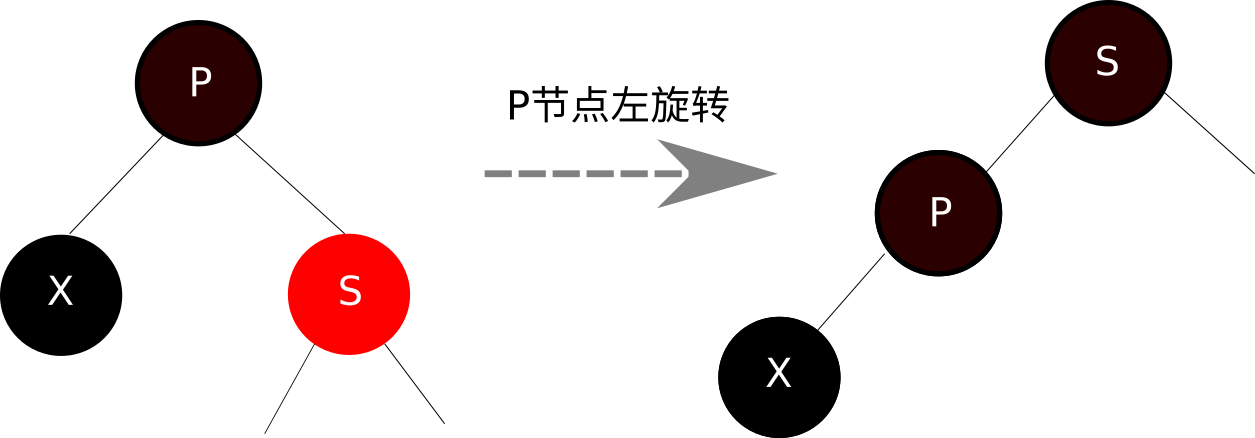
\includegraphics[width=5cm, height=1.8cm]{images/delete_fixup_red_brother.png}
		\caption{兄弟节点为红色}
		\label{fig:delete:red:brother}
		\end {subfigure}
		
		\begin{subfigure}{\textwidth}
			\centering
			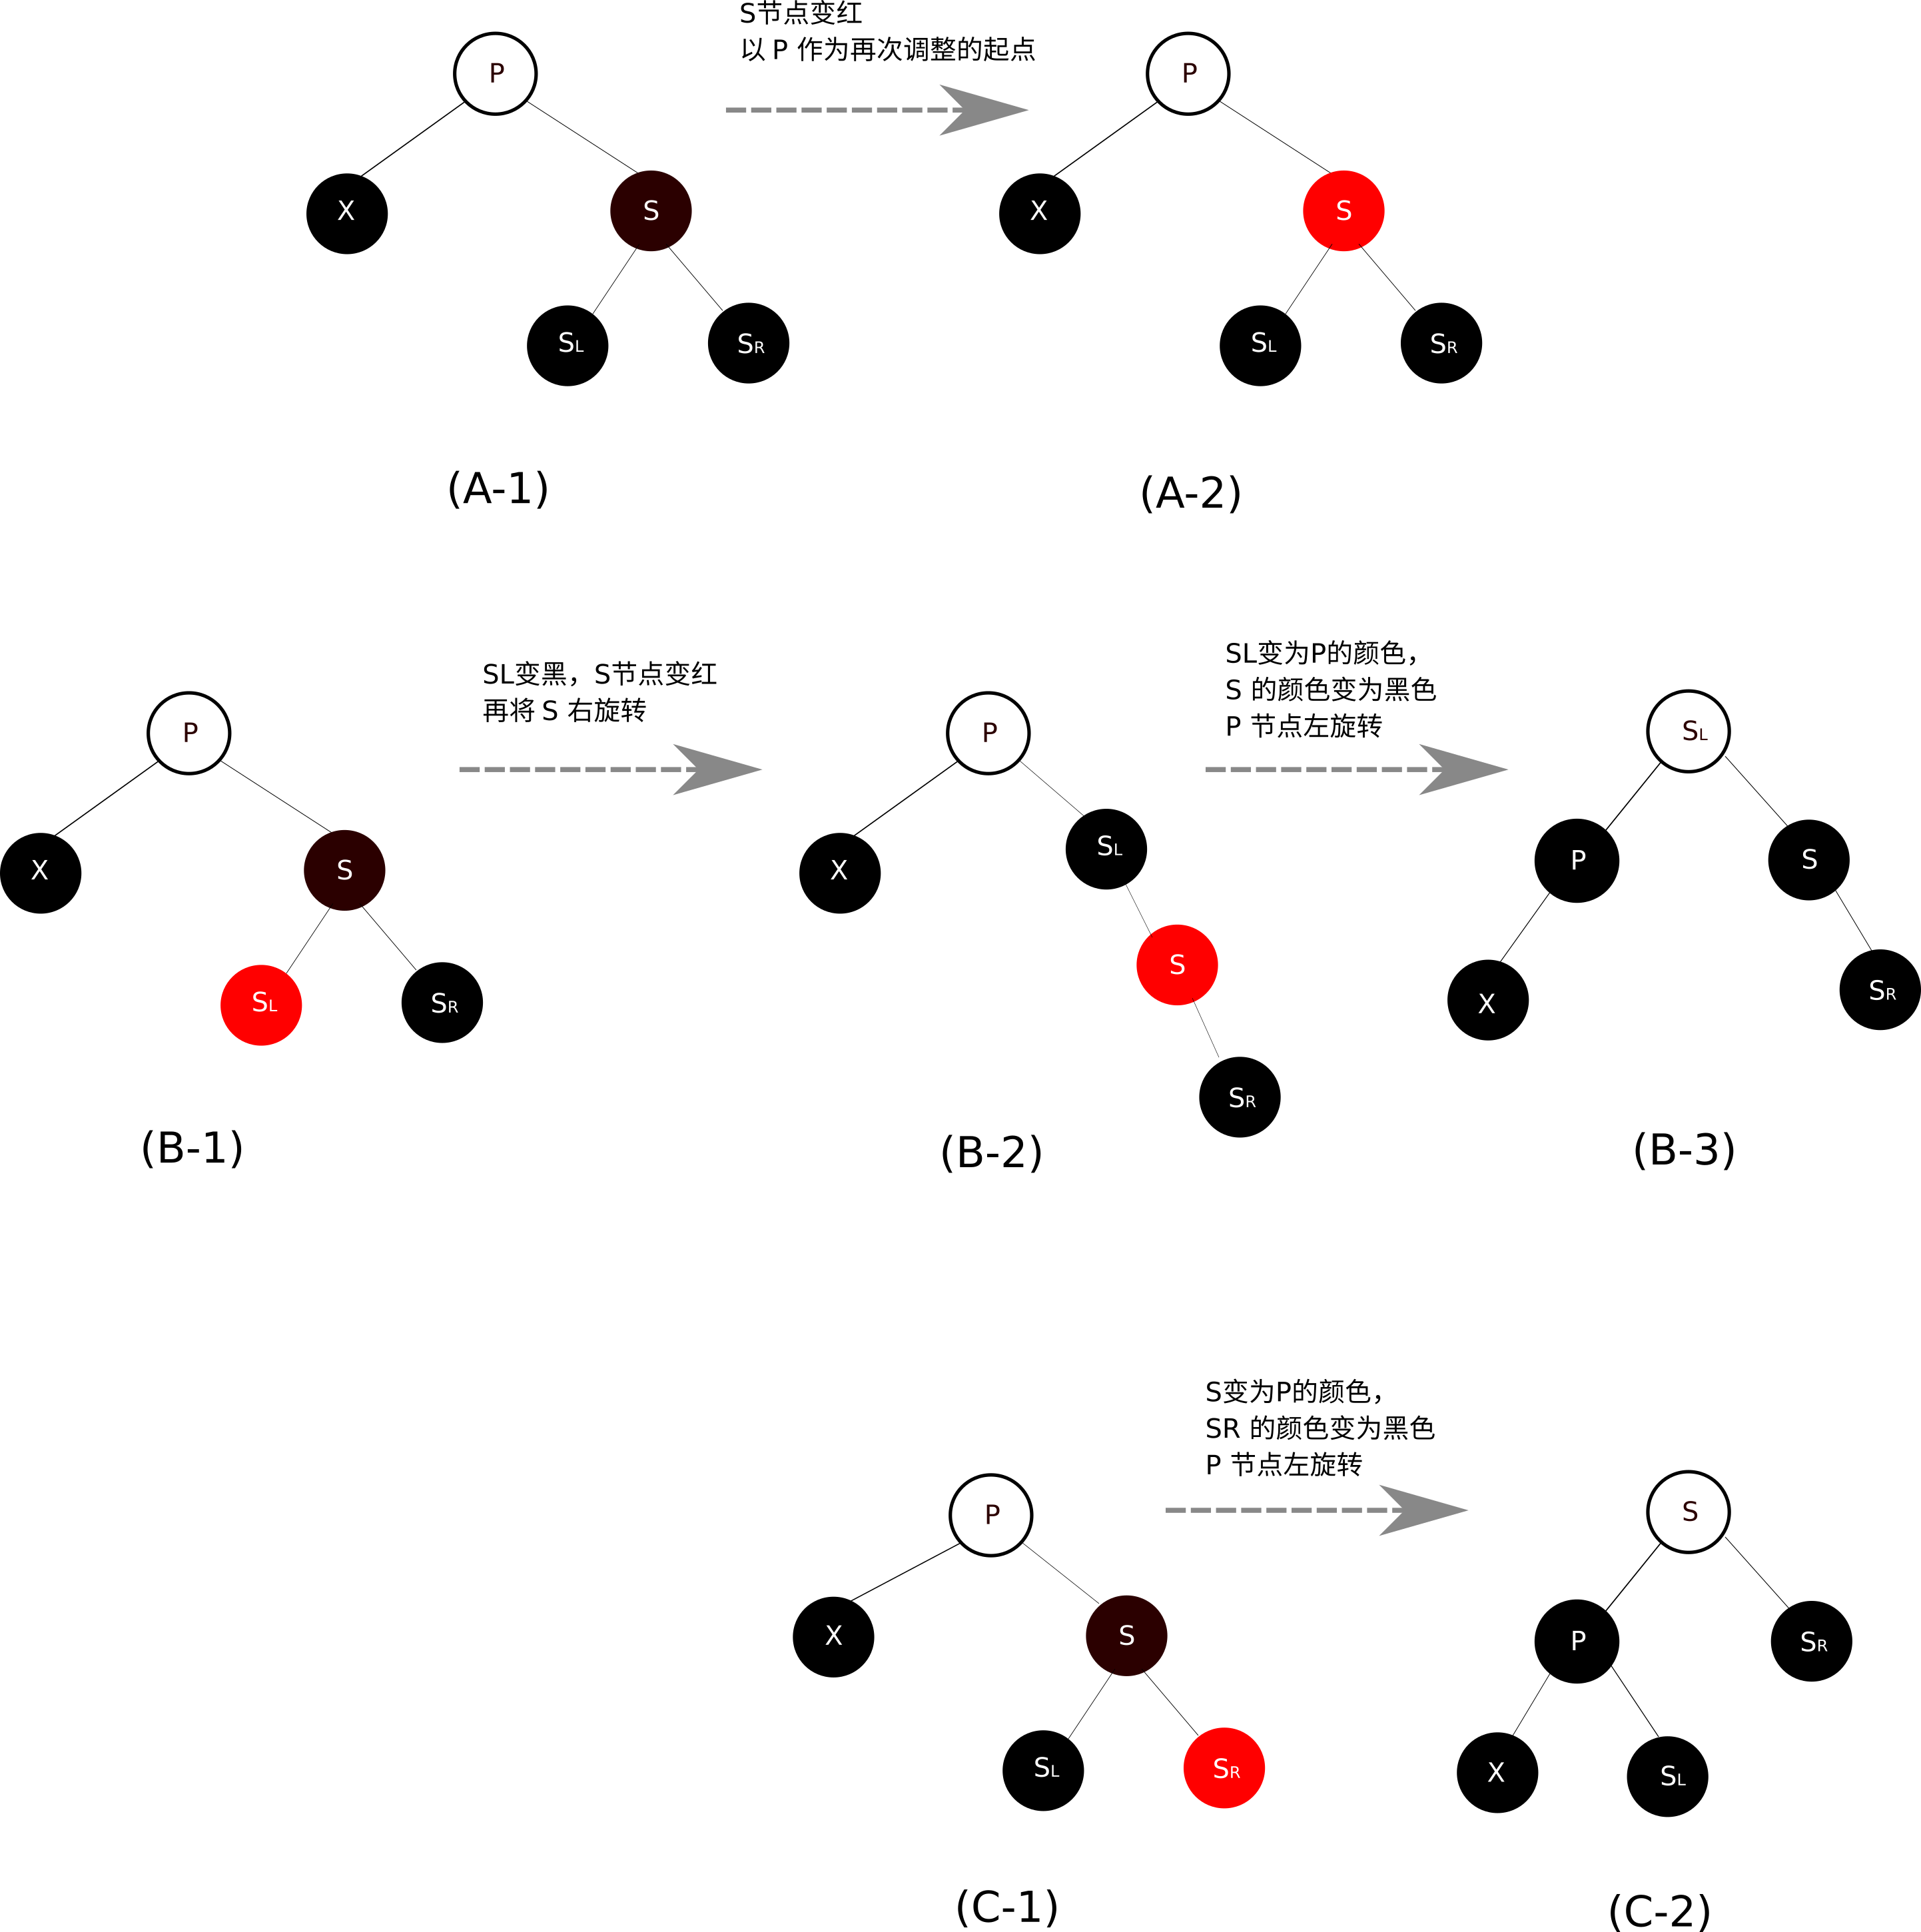
\includegraphics[width=9cm,height=9cm]{images/delete_fixup_black_brother_tree.png}
			\caption{兄弟节点为黑色}
			\label{fig:delete:black:brother}	
		\end{subfigure}
		
		\caption{删除后恢复性质过程}
		\label{fig:delete:fixup}
	\end{figure}

首先明确:调用 \verb|RB-DELETE-FIXUP(T, x)| 前,出现的问题就是黑色节点 y 被摘除了,黑高少了一!\par

理解删除后恢复红黑树性质的操作,费了不少力气,算法导论中讲述说,弄个虚拟的额外的黑色给 x $\cdots$,看得
我更难理解$\cdots\cdots$
整理学习笔记时,我以为我完全弄明白了。但我发觉无法按伪代码来逐段描述,一描述就陷
进去,乱得不清楚伪代码是要做什么了。
后来在写实现代码时,换了个方式来想,这些伪代码段要在处理什
么样的情况,才逐渐明朗,最终绘成了图片\ref{fig:delete:red:brother}与
\ref{fig:delete:black:brother}(为了便于跟踪节点是如何旋转调整的,节点的
字母我没变动):



图\ref{fig:delete:red:brother} 的情况是兄弟是红的,由性质\ref{prop:four}、
性质\ref{prop:two}推出父肯定存在,而且是黑色的。所要
做的就是挪父节点 P 去补回缺失的黑高:红兄弟 S 变黑,右旋转P节点,使得P补回缺失的黑高去了,S又刚好顶
替了 P 的位置。重新平衡!完工。

图\ref{fig:delete:black:brother} 的情况是兄弟是黑的,由于被删除的 y 节点也是黑的,P 节点的颜色
无法确定,
但依然无法阻挡红黑树的发明者(等你弄明白了红黑树结构,想必也会
惊叹发明者思想的精妙)。此情况下,要看看S的子节点有没有可以利用的红节点,

\begin{enumerate}
\item A 行的图,表明 S 没有红色子节点,没办法在 P 子树内自行恢复红黑树性质,
只好S变红,将 S 子树也自减一个黑高,现在 P 左右是平衡了,但 P 子树仍然少一个黑高!
所以,以 P 为新的起点,再循环,好向上层寻求调整。就会出现以下三种可能:

\begin{itemize}
\item 如果 P 是黑的,以 P 为新的调整起点,循环重复调整过程。
\item 如果 P 已经是树根,此时,树根左右已经是平衡的了,循环结束。
\item 如果 P 是红的,循环结束,FIXUP 函数返回时将 P 变黑(第23行),平衡了!
\end{itemize}

\item B 行的图,S 的左孩子 $S_L$ 是红的, 则将 S 变红,$S_L$ 变黑, 右旋转 S,将 $S_L$ 顶替
S 的位置。再将 $S_R$ 使用 $S_L$ 的颜色(黑色),$S_L$ 使用 P 的颜色,P 变黑,左旋转 P,
现在 P 补回了被删除的黑高,原来的兄弟子树性质也没变!完工。

\item C 行的图,S 的右孩子 $S_R$ 是红的, 去除图中节点标记的字母,只看颜色,是不是跟上述 B 行
的右旋转 S 之后的情况一样了?\footnote{
等我画完\ref{fig:delete:black:brother}的图,我算是意识到了为什么看别人的资料那么难,包括那本
书,是因为有些资料将几种情况试图最终汇集成一种
情况,所以,就看到了那些标记节点的字母在各个节点间飞来飞去。那本算法书上还介绍说假定 X 节
点还有额外的一重黑色,以抵上被删除的黑高,然后目的就成了找一个节点来抵销这个``额外‘’的一
重黑色,在刚开始学、没理解这个算法前,像我这样的理解能力,觉得这样的描述真是加重了复杂
程度!更难理解。}

\end{enumerate}


\subsection{删除操作一系列旋转、变色,究竟有没有动到了 NIL 叶子节点?}
可能有!但也仅是变更其指针指向某个节点。从始至终,颜色是肯定没有被改成红色的。

\section{删除节点后恢复性质操作总结}

真正被删除节点(y)有没有导致黑高少一,不少不用调整;
如果要调整,补上真正被删除的节点位置的节点(x)能不能也补回这个黑高?能就不用继续。
否则,看看兄弟子树那边能不能挪一个红节点出来顶替父节点,这样父节点就可挪去补回缺少的黑高;
如果也不能,兄弟子树也自己减少一个黑高,以父节点作为新起点,重复调整过程。\newline

总的来说,尽量小范围内解决性质被破坏问题,不能解决再向上层寻求。

\newpage
\begin{thebibliography}{99}
\bibitem{algorithm:intro}机械工业出版社:算法导论(第3版),中译版,2015
\bibitem{book:solution}http://www2.imm.dtu.dk/~phbi/files/teaching/solution.pdf
\bibitem{rbtree:visual}可视化的红黑树操作(注意它的删除操作是找前继的)https://www.cs.usfca.edu/~galles/visualization/RedBlack.html
 
\end{thebibliography}
\end{document}
